% This is the chapter where all the TPCN on Cu(111) related stuff goes into:
TPCN is evaporated for \SI{80}{\minute} at \SI{490}{\degreeCelsius} onto the copper surface held at room temperature. After dosage, the sample is cooled down to \SIrange{5}{7}{\kelvin} and investigated in STM. The density  is \SI{47.5E15}{} molecules per square meter - 47500 molecules / square micrometer.

\paragraph{chain motiv}
TPCN forms chains and islands with no long range order on the copper surface. Within the chains, one side of each molecule (the tips of two neighbouring legs) point to the tips of the adjacent molecule's legs. When initially formed on the copper surface, these chains are 3 to 4 molecules long.

A more detailed look shows that the chains are oriented on the copper surface with preferred direction. After room temperature deposition, the chains build up in directions \SI{30}{\degree} rotated compared to the close packed row directions of the copper crystal - right so in between them.

\begin{figure}[!h]
 \subfigure[Molecules adsorbed on Cu(111) at room temperature]{
 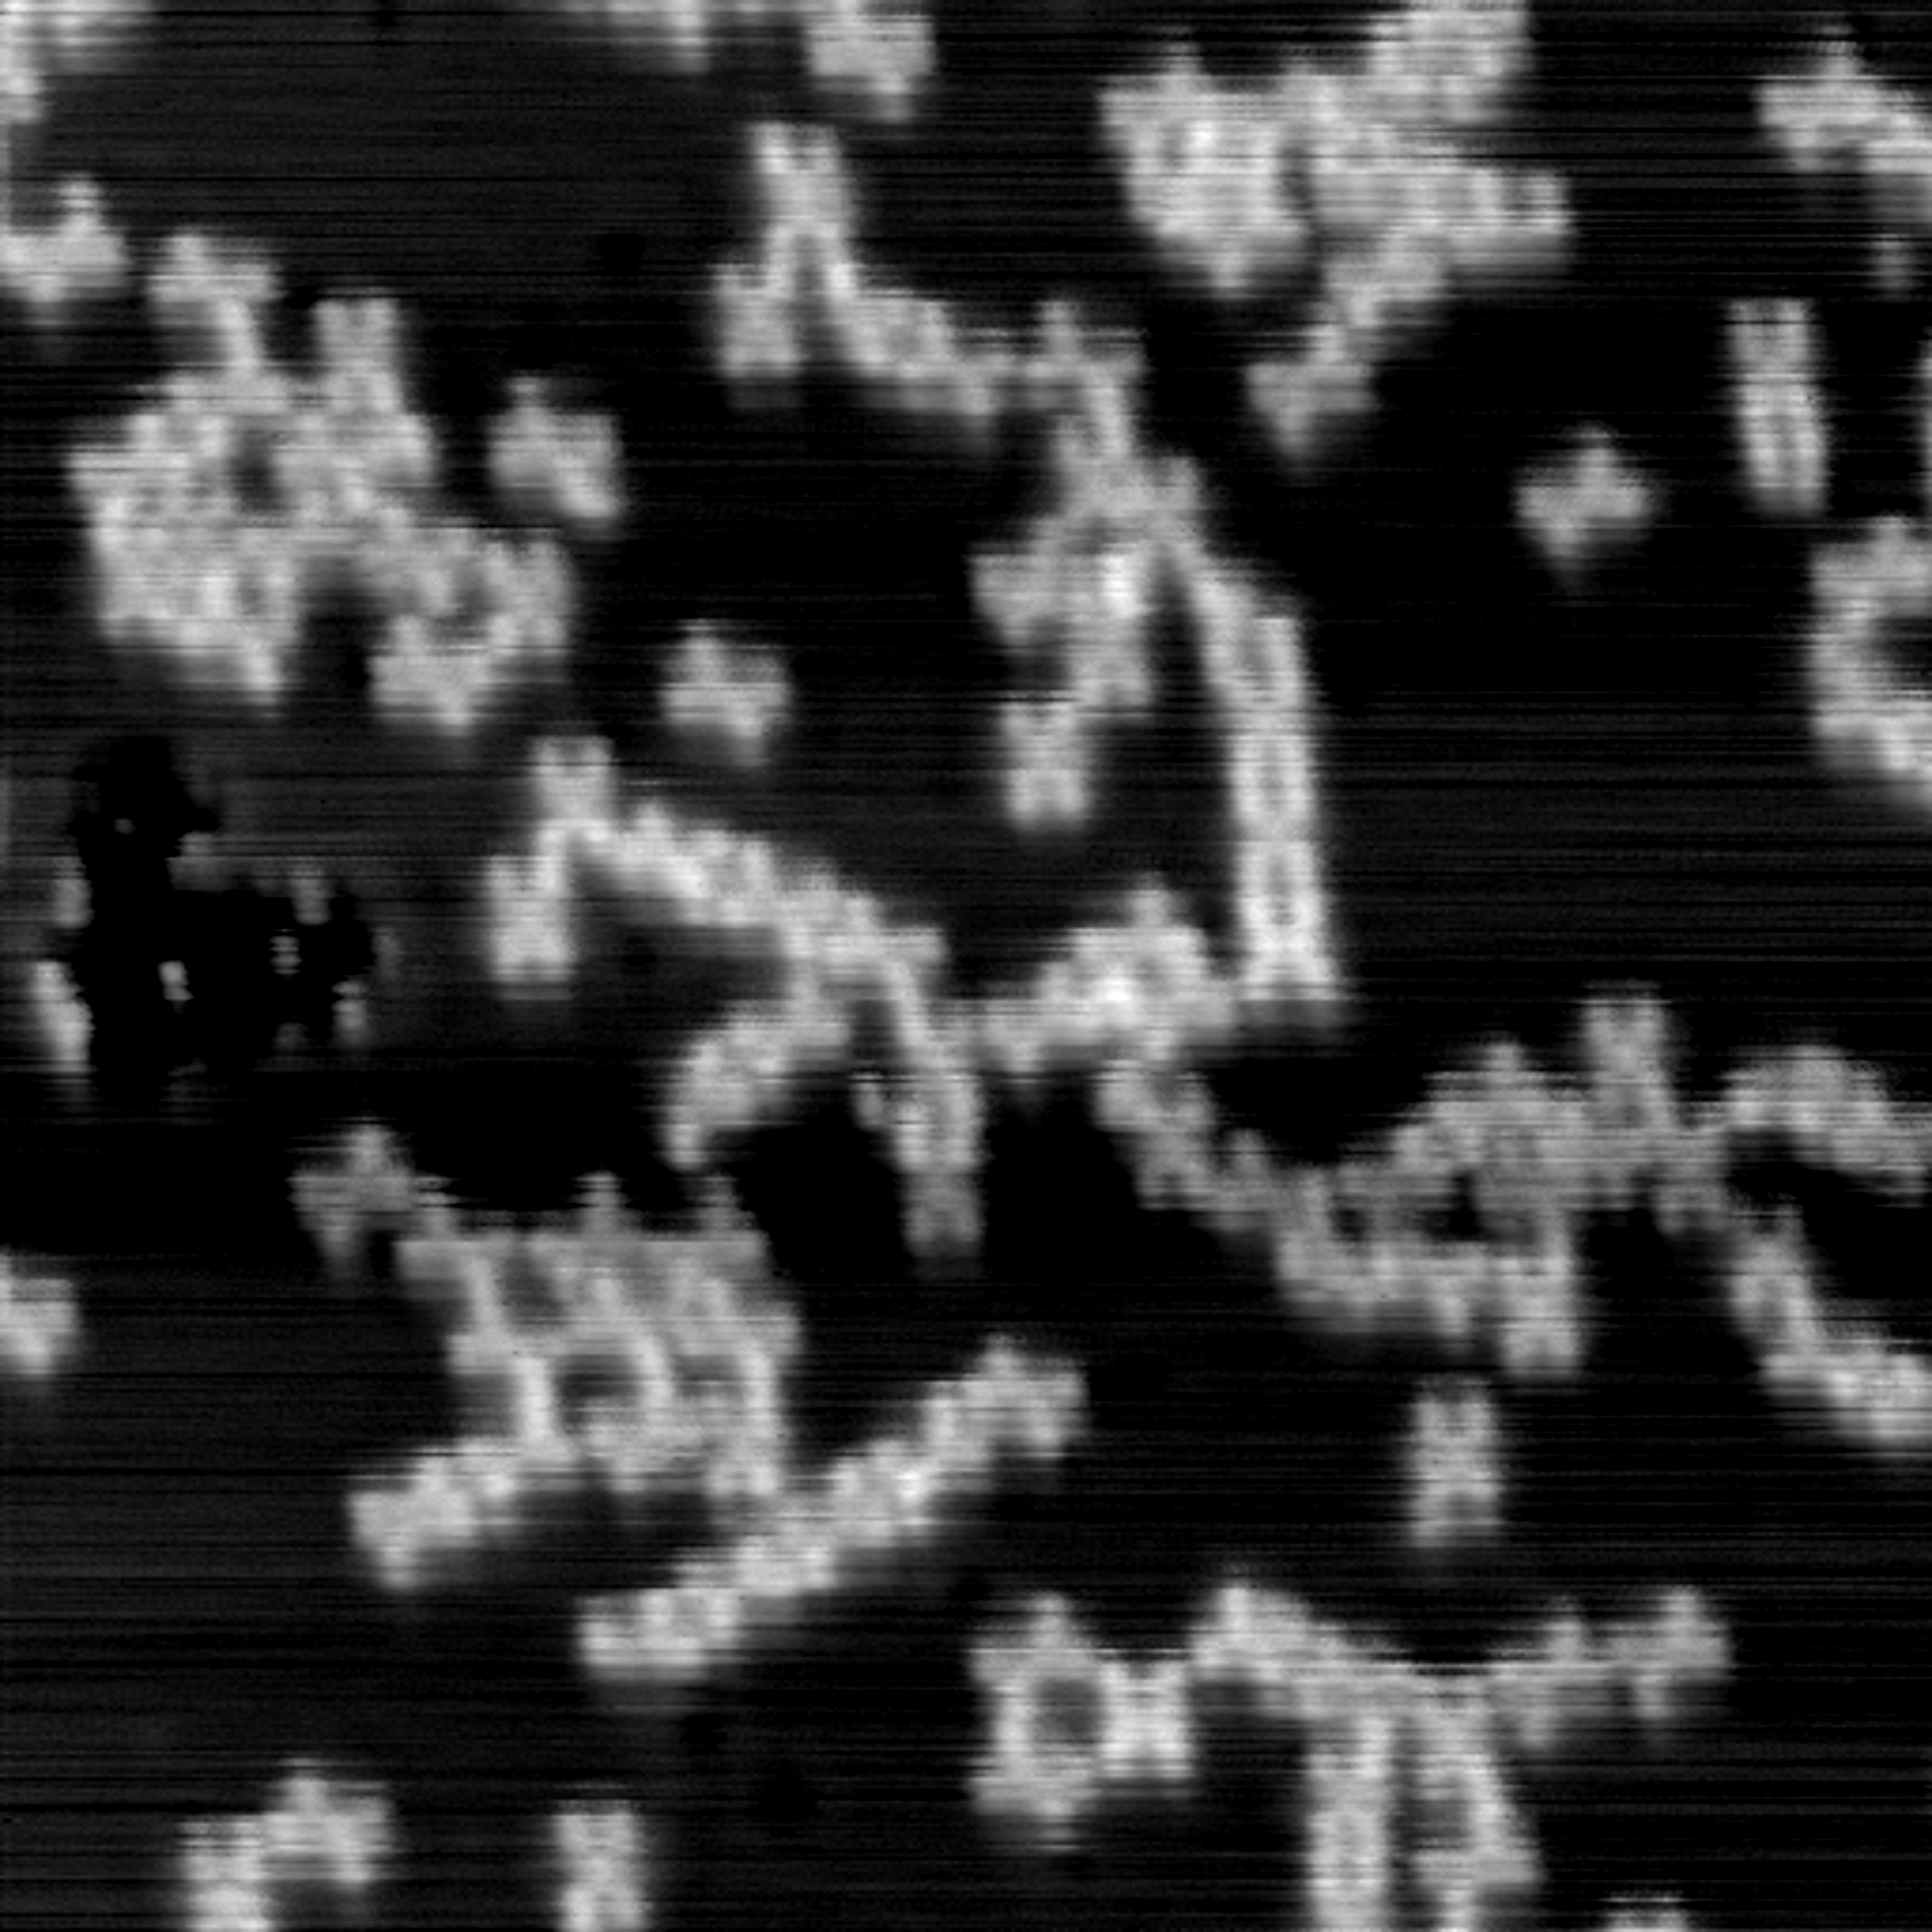
\includegraphics[width=0.45\textwidth]{./images/F150804-133056}
 }
 \subfigure[The same preparation heated to \SI{120}{\celsius}]{
 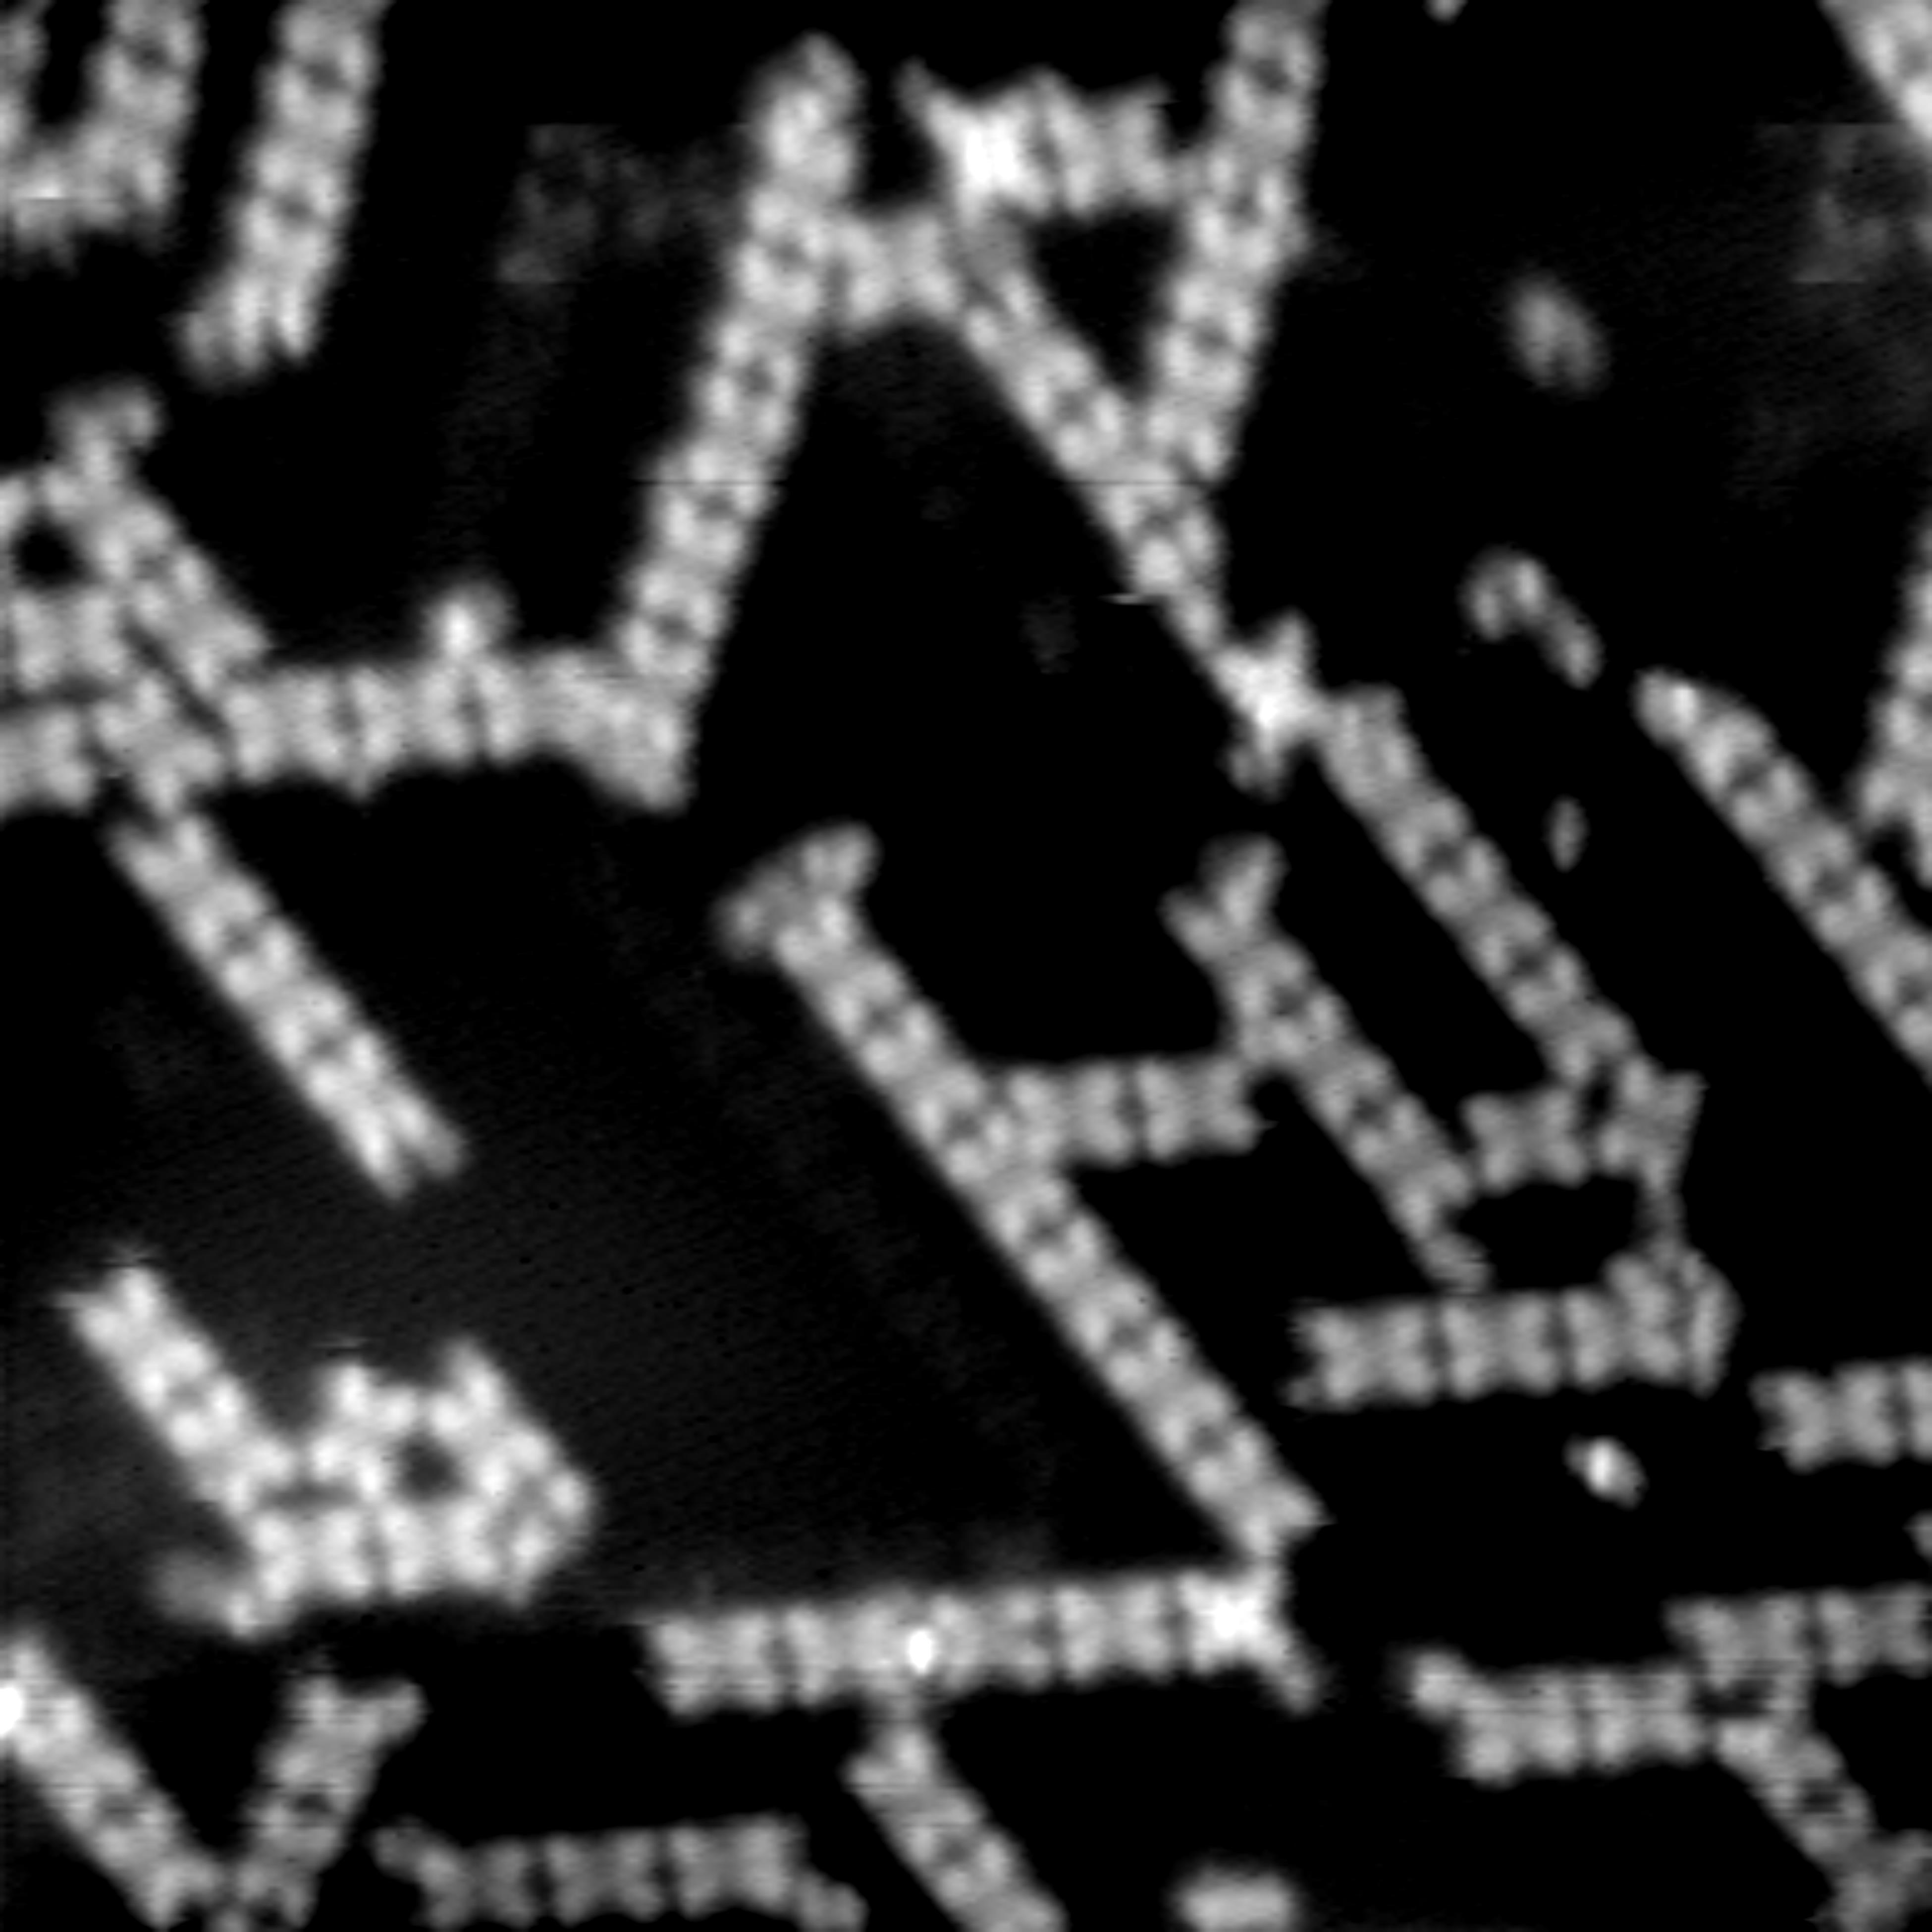
\includegraphics[width=0.45\textwidth]{./images/F150805-145931}
 }
 \caption{Preparation of \SI{47.5E3}{\per\square\micro\meter} molecules of TPCN on the (111) copper single crystal facet.}
\end{figure}

After short annealing to \SI{120}{\celsius} for \SI{10}{\minute} the length and orientation of the chains changes. The length increases to a typical length of \SIrange{3}{6}{molecules}. The direction also changes - now all orient along the direction of close packed surface atoms.
A much higher fraction of deposited molecules arranges in chains, only some of the molecules still form unordered islands.

\paragraph{bended or twisted?}
As one can see in the images, the geometry of the majority of molecules changes upon adsorption on the metal surface.
When calculated for optimum geometry (AM1) in gas phase (with Hyperchem), they appear as squares. The molecules that build up the chain look not square anymore but instead rectangular. Chain direction is defined parallel to the longer side of the rectangle.
The angle between two TPCN-legs is about \SI{68}{\degree} (\SI{112}{\degree} respectively) in the STM images. There are two possible explanations for this change.
\begin{itemize}
 \item The whole leg of the molecules is rotated, reducing the angle between both. It may be possible, that the saddle-shaped macrocylce deforms in such a way that the inner phenyl ring of the legs (in gas phase already rotated by \SI{45}{\degree} with respect to the plane of the macrocycle - elevation angle) may avoid steric hinderance. Only a small additional rotation of \SI{10}{\degree} (azimuth) would be needed for each leg to make the geometry match the observed motivs.
 \item Rotation of a single phenyl ring within the leg can attribute the sheared look of the legs. STM is more sensible to the higher parts of the phenyl ring (remember: rotated by \SI{45}{\degree}, there is a higher and a lower part), this would not be on the line linking the end of leg and the macrocycle, but slightly off. If more phenyl rings are rotated towards each other the apparent angle between the legs is reduced, while only the phenyl rings are rotated. 
\end{itemize}
\emph{Add some illustration here - this angles get confusing :D}
\begin{figure}
 \centering
 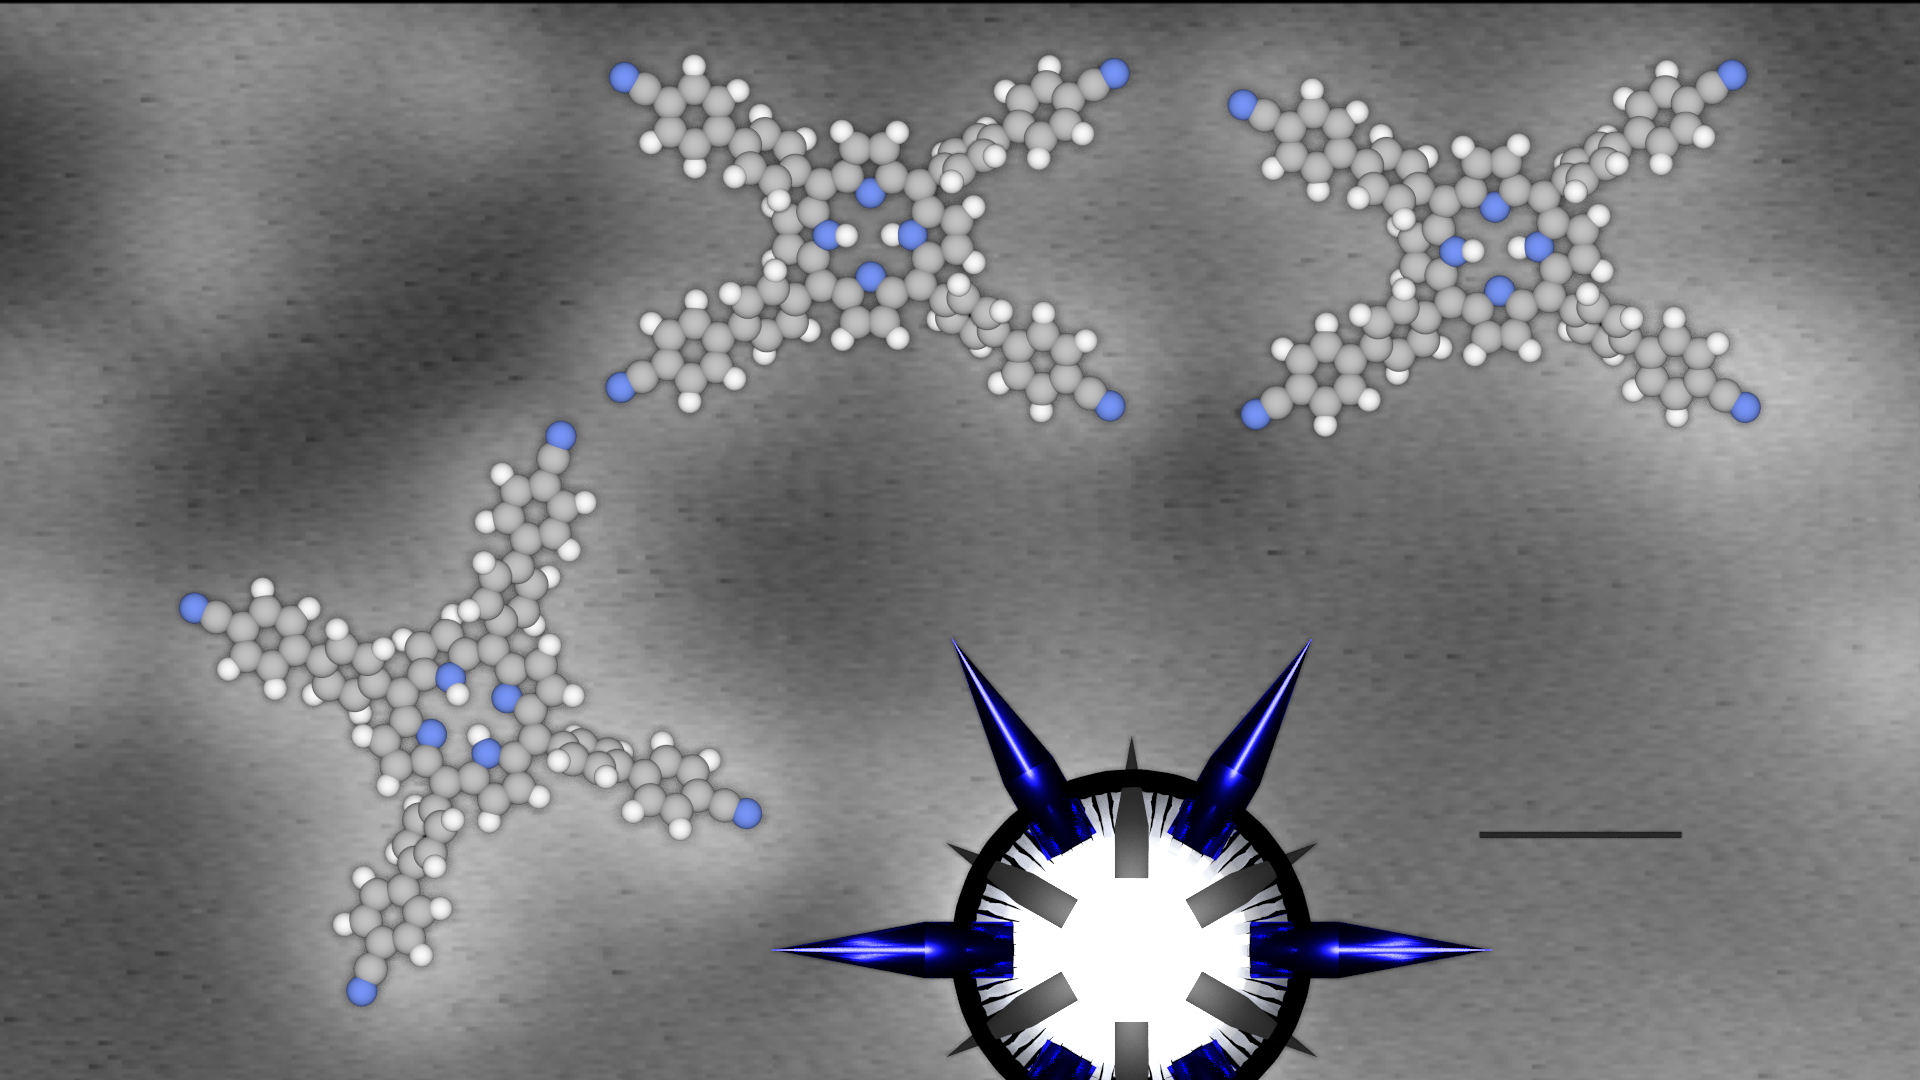
\includegraphics[width=0.49\textwidth]{./images/F150816-162243}
 \caption{Molecules deform upon adsorption on copper}
\end{figure}

\paragraph{binding}
\label{chapter:TPCN-adatoms}
Regardless of the actual orientation of the legs a center-center distance of two molecules in a chain can be measured. Typical center-center distances between two molecules within chains are \SI{2.7}{\nano \meter}.
The above mentioned leg twisting mechanism then results in different distances between the endpoints of a TPCN leg between two adjacent molecules in a chain. 

If the molecules were to adsorb in a gas-phase-like configuration, the distance between the centers of the two nitrogen atoms at the legs end is about \SI{6.9}{\angstrom}. When the legs are bended by \SI{10}{\degree}(to match the STM image), this distance is reduced to \SI{3.76}{\angstrom}.

Further more, a copper atom may be present or not to mediate the bond between the two nitrogens. Although no direct adatom could be observed in STM, this type of binding is often observed [citations: yuanchins master thesis]\cite{klappenberger_temperature_2008}. Typical N-Cu binding distances of \SI{2}{\angstrom} are reported in literature\cite{klappenberger_temperature_2008}, and range up to \SI{3}{\angstrom} for Cu-carboxylate systems on Cu(111)\cite{classen_templated_2005}. So for both possible scenarios (bended legs, rotated phenyl ring) both N-N distances (\SI{3.8}{\angstrom},\SI{6.9}{\angstrom}) reflect possible N-Cu binding distances (\SI{1.9}{\angstrom},\SI{3.45}{\angstrom}) in the reported ranges, although the N-Cu distance (\SI{1.9}{\angstrom}) for the bended legs matches better. 
Systems with copper dimers mediating the molecular connection are reported too\cite{lin_real-time_2002}.

These findings are supported by similar reports on similar functional groups [citations: yuanchins master thesis p 65/66]. The position of the copper atom itself can only be estimated. Either it is right between the two nitrogen atoms, or it is slightly further away at the (imaginary) connection point of the (imaginary extended) legs. The tradeoff between N-Cu-N binding strength and Cu-Cu binding force determines the position of the copper adatom.

\paragraph{Cu-foil}
The buildup of chains is much more prohibited on the copper foil - either because the molecules aren't able to move (pinned to impurities, contrained movement given by facettet surface). In case of the copper mediated bonding the adatom-density than could be lower than in the single crystal case and the formation of chains is suppressed.